\newpage
\subsection{}

Economics is math driven.
It is used to describe the real world with models.

\begin{definition}
    \emph{Functions} can be expressed in words, tables, equations or graphs.
\end{definition}
\begin{figure}[h!]
    \centering
    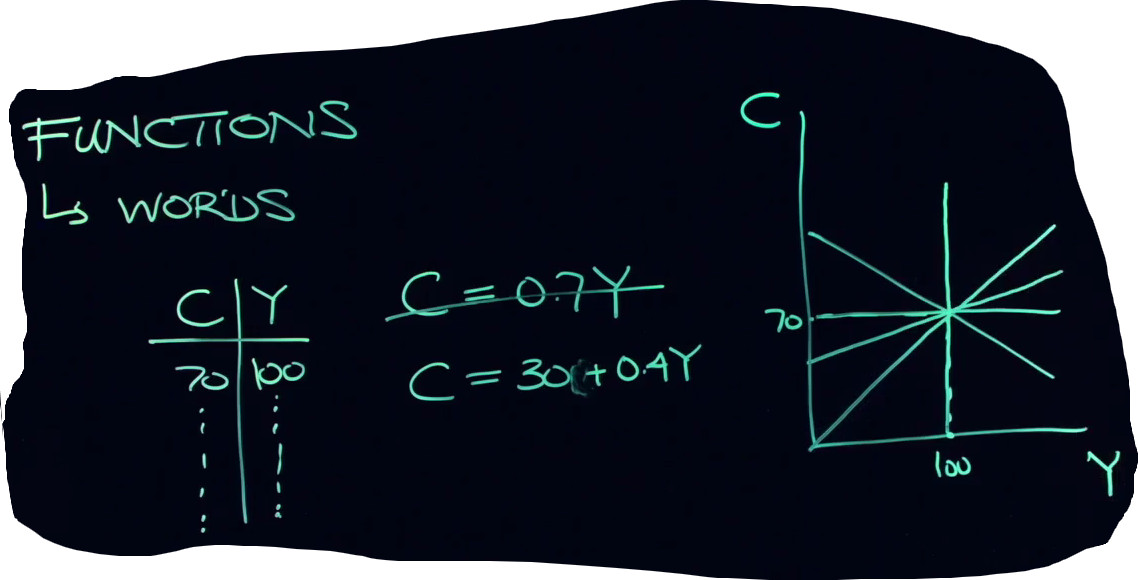
\includegraphics[width=0.75\textwidth]{Chapter2/RepresentationsofFunctions.png}
    \caption{Different Representations of Functions}
\end{figure}
Most of what is done in intro to economics is done with linear functions.
Non-linear functions are interesting because they can be used to find maximum and minimums (optimization).